

\section{Implementation}
\label{sec:implementation}

The implementation..

\begin{enumerate}
	\item The extra things we did to make the thing actually run
	\item Code architecture
	\item Optimizations
\end{enumerate}


\begin{figure}[htbp]
	\centering
	
	% Top row: (a), (b), (f)
	\begin{subfigure}[b]{0.45\textwidth}
		\centering
		\includegraphics[width=\textwidth]{plots/bidirectional_pruning_step_a_init.pdf}
		\caption{Step (a)}\label{fig:step:a}
	\end{subfigure}\hfill
	\begin{subfigure}[b]{0.45\textwidth}
		\centering
		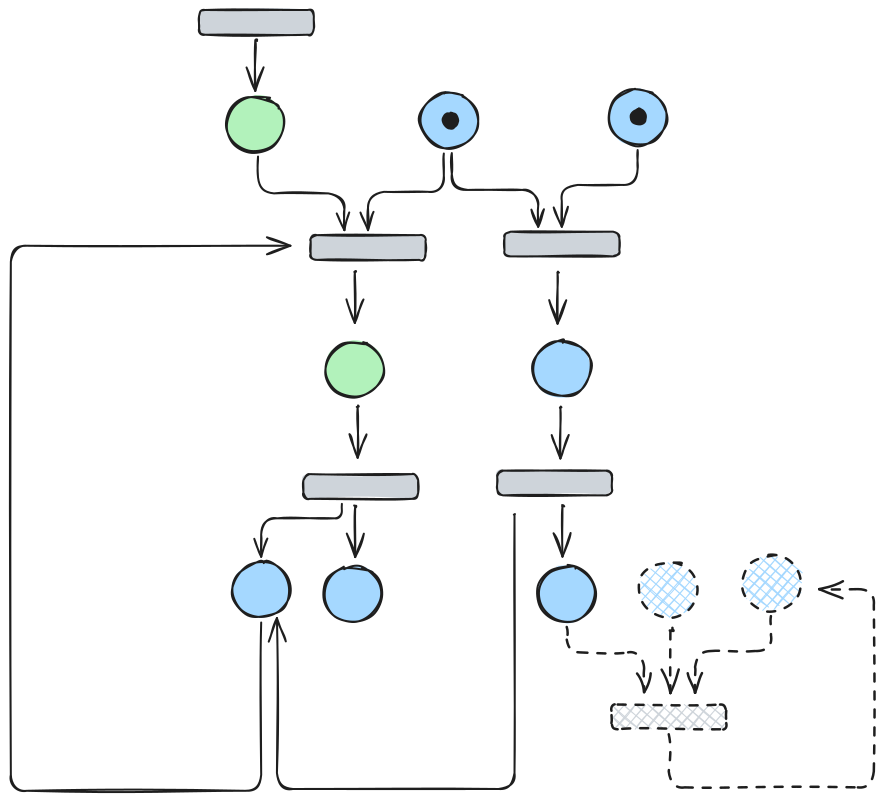
\includegraphics[width=\textwidth]{plots/bidirectional_pruning_step_b_forward.pdf}
		\caption{Step (b)}\label{fig:step:b}
	\end{subfigure}\hfill
	
	
	\vspace{1em}
	
	% Bottom row: (c), (d), then stacked (e)/(f) slot
	\begin{subfigure}[b]{0.30\textwidth}
		\centering
		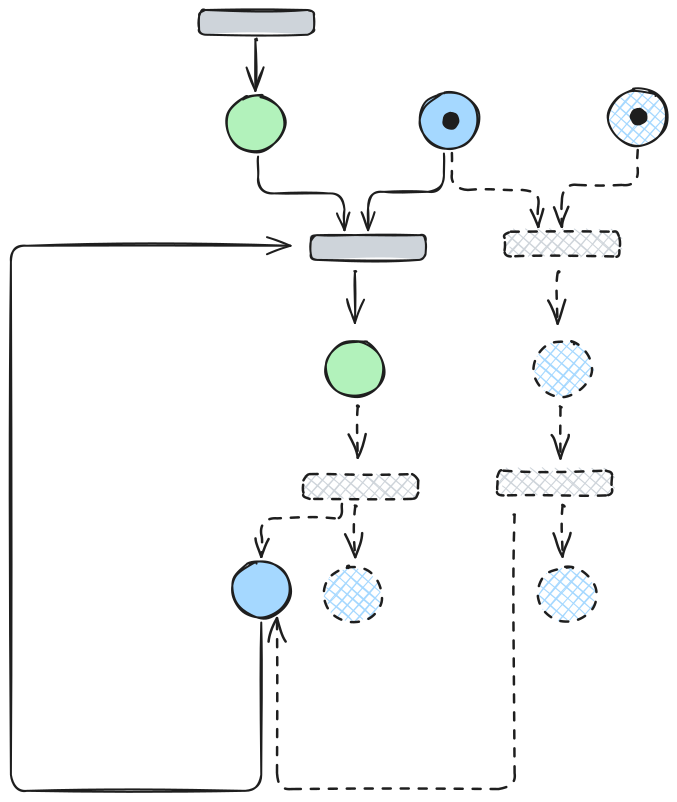
\includegraphics[width=\textwidth]{plots/bidirectional_pruning_step_c_backward.pdf}
		\caption{Step (c)}\label{fig:step:c}
	\end{subfigure}\hfill
	\begin{subfigure}[b]{0.23\textwidth}
		\centering
		\includegraphics[width=\textwidth]{plots/bidirectional_pruning_step_d_forward.pdf}
		\caption{Step (d)}\label{fig:step:d}
	\end{subfigure}\hfill
	\begin{subfigure}[b]{0.23\textwidth}
		\centering
		% nested for (e)
		\begin{subfigure}[b]{\textwidth}
			%	       \vspace{-0.5ex}  
			\raisebox{17ex}{%
				\includegraphics[width=0.65\textwidth]{plots/bidirectional_pruning_step_e_backward.pdf}%
			}
			%		\captionsetup{skip=-15.5ex}
			\caption{Step (e)}\label{fig:step:e}
		\end{subfigure}
		
		\vspace{0.5em}
		
		% nested for (f)
		\begin{subfigure}[b]{\textwidth}
			\centering
			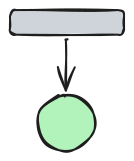
\includegraphics[width=0.23\textwidth]{plots/bidirectional_pruning_step_f_final.pdf}
			\caption{Step (f)}\label{fig:step:f:bottom}
		\end{subfigure}
	\end{subfigure}
	
	\caption{All six bidirectional‐pruning steps, with (e) and (f) stacked in the same column.}
	\label{fig:bidirectional_pruning}
\end{figure}




\newpage